\section{Implementación de Flip Flop y Latch}

En esta sección se propone la implementación de un flip flop de tipo
''D'' y de un latch ''SR'' a partir de compuertas lógicas discretas.

\subsection{Latch SR}

Para realizar el latch SR se propuso el siguiente diseño:

\begin{figure}[H]
\centering
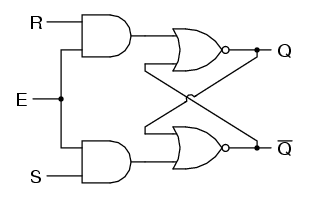
\includegraphics[scale=0.5]{./circuitoLATCH.PNG}
\caption{Diseño de Latch SR}
\end{figure}

Una vez materializado el latch, se procedió a medir algunos parámetros
de interés, los cuales se constrastaron con parámetros comerciales:

\begin{table}[H]
    \centering
\begin{tabular}{|c|c|c|c|c|}
\hline 
Parámetro & Desde & Hasta & Medido & Hoja de Datos (valores típicos)\tabularnewline
\hline 
\hline 
Tpropagación & S & Q & 24 ns & 15 ns\tabularnewline
\hline 
Tpropagación & R & Q & 28 ns & 15 ns\tabularnewline
\hline 
\end{tabular}

\caption{Comparación con Latch Comercial}
\end{table}

Vale aclarar que los parámetros del latch comercial fueron extraídos
de la hoja de datos del 74LS279.

\subsection{Flip Flop D}

Para la realización del flip flop D se propuso el siguiente diseño:

\begin{figure}[H]
\centering
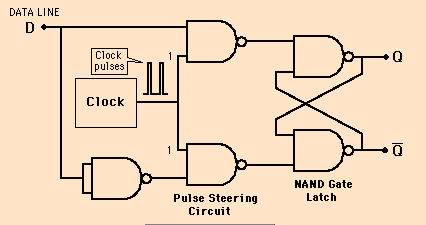
\includegraphics[scale=0.5]{./circuitoFLIPFLOP.PNG}
\caption{Diseño de Flip Flop D}
\end{figure}

Luego de la materialización del flip flop se procedió a medir algunos
parámetros de interés, los cuales se constrastaron con parámetros
comerciales:

\begin{table}[H]
    \centering
\begin{tabular}{|c|c|c|c|c|}
\hline 
Parametro & Desde & Hasta & Medido & Hoja de Datos (valores típicos)\tabularnewline
\hline 
\hline 
TpropagaciónHL & clock & Q & 31 ns & 10 ns\tabularnewline
\hline 
TpropagaciónLH & clock & Q & 29 ns & 10 ns\tabularnewline
\hline 
\end{tabular}

\caption{Comparación con Flip Flop Comercial}
\end{table}

Débese aclarar que los parámetros del flip flop D comercial fueron
extraídos de la hoja de datos del 74LS74.

Con respecto a los resultados obtenidos, las mediciones muestran que
los tiempos de propagación al realizar el flip flop o el latch con
compuertas discretas aumentan con respecto a los tiempos de propagación
que presentan los comerciales. Esto es razonable ya que en la implementación
con compuertas discretas se utilizan más componentes que influyen
en el retardo de la señal.